\documentclass{article}

% if you need to pass options to natbib, use, e.g.:
%     \PassOptionsToPackage{numbers, compress}{natbib}
% before loading neurips_2021

% ready for submission
\usepackage[preprint]{neurips_2021}

% to compile a preprint version, e.g., for submission to arXiv, add add the
% [preprint] option:
%     \usepackage[preprint]{neurips_2021}

% to compile a camera-ready version, add the [final] option, e.g.:
%     \usepackage[final]{neurips_2021}

% to avoid loading the natbib package, add option nonatbib:
%    \usepackage[nonatbib]{neurips_2021}

\usepackage[utf8]{inputenc} % allow utf-8 input
\usepackage[T1]{fontenc}    % use 8-bit T1 fonts
\usepackage[colorlinks=true]{hyperref}       % hyperlinks
\usepackage{url}            % simple URL typesetting
\usepackage{booktabs}       % professional-quality tables
\usepackage{amsfonts}       % blackboard math symbols
\usepackage{nicefrac}       % compact symbols for 1/2, etc.
\usepackage{microtype}      % microtypography
\usepackage{xcolor}         % colors
\usepackage{graphics}       % include graphics
\graphicspath{ {./fig/} }   % standard path to image folder
\usepackage{float}

\title{Analyzing the Effects of Different Features\\ on Remote Workers' Salaries}

% The \author macro works with any number of authors. There are two commands
% used to separate the names and addresses of multiple authors: \And and \AND.
%
% Using \And between authors leaves it to LaTeX to determine where to break the
% lines. Using \AND forces a line break at that point. So, if LaTeX puts 3 of 4
% authors names on the first line, and the last on the second line, try using
% \AND instead of \And before the third author name.


\author{%
  Tim Weisbarth\\
  Matrikelnummer 5673676 \\
  \texttt{tim.weisbarth@student.uni-tuebingen.de} \\
  \And
  Manuel Arns\\
  Matrikelnummer 6088776\\
  \texttt{mail@manuelarns.de} \\
}

\begin{document}

\maketitle

\begin{abstract}
    %TODO
    % regression graph: IMO red dots darker

    This report is an analysis of how features like company size, work experience, company location, a countries GDP and remote ratio affect the salaries of remote workers, using a dataset by foorilla LLC \cite{datasets2022}. The used methods are the Spearman correlation coefficient, linear regression, and choropleth maps. The results show that the GDP as well as the experience level of a worker seem to have the highest influence on the salaries with a coefficient of determination of the regression of $R^2=0.52$. All code can be found in our \href{https://github.com/manuelarns/Data-Literacy-Project}{GitHub repository}.
    
\end{abstract}

\section{Introduction}
There are many reasons why workers are paid the way they are. One might have certain assumptions of what factors have the biggest effect on a job's salary; however, these may not hold true. Especially remote desk jobs have many factors that may determine what a worker's labor is worth. This report is an attempt to find these most influential predictors for remote work salaries, using the remote work salaries dataset by "foorilla LLC" \cite{datasets2022}. For this a data analysis pipeline, comprised of data collection, preprocessing, analysis, and visualization, is used. The following sections describe the pipeline in more detail. After this, the analysis results are discussed and put into context.

\section{Data Collection}
The data is continuously being collected by a company called "foorilla LLC" within the "Fresh Remote Work salaries" project. The projects' website states: "This site collects salary information anonymously from professionals all over the world in the Remote Work space and makes it publicly available for anyone to use, share and play around with." Anyone, willing to share their salary information, can fill out the form on the website. There are several reasons however, to be wary about the provided remote salary dataset. Firstly, it is unclear how careful users filled out the forms and how "foorilla LLC" preprocesses this input data before providing it on their website. Secondly, foorilla LLC has three additional salary data collection websites (namely AI-Salaries, Cyber-Security-Salaries, DevOps-Salaries) \cite{datasets2022}. Our experiment shows that each of these sites has a more than than 50\% overlap with the remote salary data, which is why the additional datasets were not used for this analysis. Thirdly, there are 45 duplicate rows in the remote dataset of which 96\% have the job title "DevOps Engineer" even though only 15\% of the rows have the job title DevOps Engineer. Lastly, the site has collected 1545 datapoints since 2020 with a sudden increase to 2451 on January 30.

\section{Data Analysis}
\subsection{Methods}
\subsubsection{Correlation Coefficient}
%The most commonly used Pearson correlation coefficient can not be applied to the dataset because not all variables are normally distributed. Instead, the Spearman correlation coefficient is used. This coefficient only requires that the correlation between two variables is monotonic and can be ranked which we assume to be the case. For any two variables $x$ and $y$ it is defined as

The most commonly used \textit{Pearson correlation coefficient} can not be applied to the dataset because not all variables are normally distributed. Instead, the \textit{Spearman correlation coefficient} is used. This coefficient only requires that all variables be rankable and the correlation between two variables be monotonic, which we assume to be the case. For any two variables $x$ and $y$ it is defined as

\begin{equation}
    r_s = \frac{\Sigma(R(x), R(y))}{\sigma(R(x)) \cdot \sigma(R(y))}
\end{equation}

where $\Sigma$ denotes the covariance, $R$ the rank, and $\sigma$ the standard deviation. It is the Pearson coefficient between the rank of the two variables \cite{spearman1904proof}.

\subsubsection{Linear Regression}
In this report ordinary least squares linear regression is used, as introduced in the lecture. It is used to analyze the influence of different features on the salaries and implemented using sklearn's LinearRegression class. In order to quantify how well this model predicts the salaries, the coefficient of determination $R^2$ is calculated. $R^2$ describes the proportion of the variance of the salaries $s_i$ which can be explained through the linear regression estimate $\hat{s_i}$. It is given by the standard formula

\begin{equation}
    R^2 = \frac{\sum_{i=1}^{n} (\hat{s_i} - \bar{s})^2}{\sum_{i=1}^n ({s_i} - \bar{s})^2}
\end{equation}

where $\bar{s}$ denotes the mean average salary and $\hat{s_i}$ the fitted value \cite{coefficient2008}. 

\subsubsection{Choropleth Map} 
We consider it likely, that the country in which a company is located could have a large impact on their employee's salary. As this information is not numeric, it cannot be analyzed with linear regression. We choose to generate a choropleth map that shows the mean average salary for each country.

\subsection{Data Preprocessing}
The salaries data contains some features that need to be preprocessed in order to fit the requirements of the analysis methods. This is done through a preprocessing pipeline. The individual steps of this pipeline are described in the following.

\textbf{Country Code Extension:}
The location information in the salary data is changed to the \textit{ISO 3166 Alpha 3} standard to match the format in the GDP data. \\
\textbf{GDP per Capita:}
Based on the GDP and population estimates provided by the world dataset, this step calculates a feature containing the GDP per capita of the country the employee resides in (from now on referred to as GDP). As this figure is generally a good indicator of a countries economical success, we suspect it to also indicate salaries.\\
\textbf{Non-Numeric to Numeric:}
The workers experience level, work year, and the companies size are are non-numeric. We assign ranks to fulfill the requirements of our correlation analysis and regression.\\
\textbf{Same Country Attribute:}
The salaries data provides both the country of residence of the employees, and the company location. This allows us to see, whether an employee works in the same country as they live. We think this could also have an impact on salary so we create a feature that encodes this binary information.\\
\textbf{AI/ML Attribute:}
We define a new attribute in the salary data, encoding whether an employee is working in an AI or ML type position or not.\\
\textbf{Outlier Detection:}
Of the employed methods, linear regression in particular is prone to be strongly influenced by outliers. To combat this we drop the top and bottom 2\% of salary data. We found this value to be a good trade-off between loss of data and improvement of analysis result.

\subsection{Results}
In this section, we discuss the results of the three conducted analyses. Figure \ref{fig:correlation} shows a heatmap containing the Spearman correlation coefficients for the salary (target) and all numeric features.

\begin{figure}[ht]
    \hspace*{-.2cm}
    \centering
    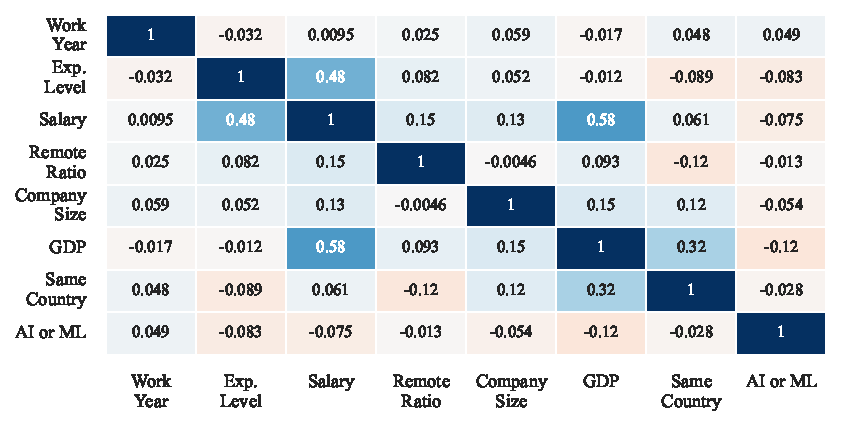
\includegraphics{correlation.pdf}
    \caption{Spearman correlation coefficients for rankable variables.}
    \label{fig:correlation}
\end{figure}

All, but the features experience level and GDP, show little correlation with the target. The correlations within the features are all below $0.15$ except for the $0.32$ correlation between the same country and GDP attribute. We assume these values to be low enough that the predictors can be regarded as uncorrelated.

The multiple linear regression (MLR) takes as predictors all attributes visible in Figure \ref{fig:correlation}. For a fair comparison, we normalize all features and calculate the regression weights. The highest are assigned to the attribute GDP at $0.55$ and "Experience level" at $0.47$, with all other weights below $0.06$. The coefficient of determination of the MLR is $R^2=0.52$.

\begin{figure}[h]
    \hspace*{-.2cm}
    \centering
    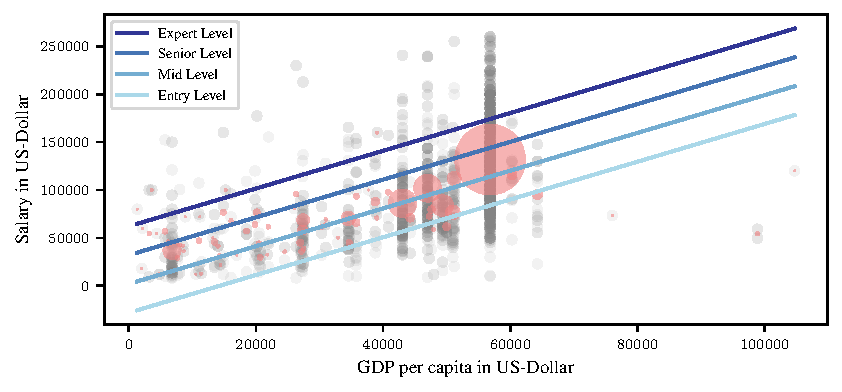
\includegraphics{regression.pdf}
    \caption{MLR results for GDP and experience level. Grey scatter: All 2248 preprocessed datapoints. Red scatter: Mean at each GDP value (area $\propto$ number of datapoints). All other predictors are set to their mean.}
    \label{fig:regression}
\end{figure}


Figure \ref{fig:regression} was created by varying the GDP for each of the four experience levels while setting all other predictors to their means, which is possible as they are regarded as uncorrelated. The vertical grey-dotted lines exist because each datapoint belongs to one country which has a unique, discrete GDP per capita. For each experience level there is a regression line. Due to the linearity of the MLR they are evenly distanced and parallel. 79 \% of the datapoints lay between a GDP of 40.000\$ and 60.00\$ with the biggest red dot at a GDP of 56.800\$ representing the 1150 datapoints from the US. This is can be an explanation for the unrealistic fit below a $0\$$ salary of the entry level regression line. 


\begin{figure}[ht]
    \hspace*{-.85cm}
    \centering
    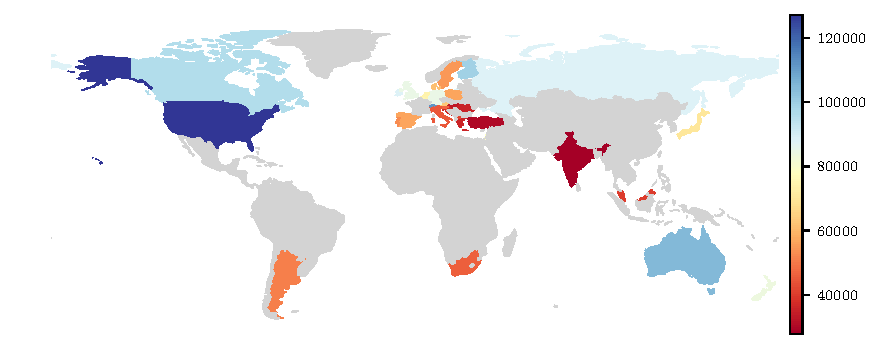
\includegraphics{choropleth.pdf}
    \caption{Choropleth map of mean average salary in USD per country.}
    \label{fig:choropleth}
\end{figure}

Figure \ref{fig:choropleth} shows the choropleth world map of mean salaries. We note that in order to have more meaningful results, we chose to eliminate all countries that have less than three datapoints. The map clearly shows the large impact the country seems to have. In general, companies in traditional western "first world" countries (e.g. USA, Canada, Australia), as well as Russia pay the highest wages. Interestingly though, the southern European nations Spain, Portugal, Italy as well as Sweden show significantly lower salaries. This gap is bigger than we expected, but could also be the cause of the extremely small sampling size. Companies in developing countries pay the lowest wages.


\section{Conclusion and Outlook}
Our results make a strong case for the country, GDP and experience as major contributors to an employee's salary; however, with $R^2=0.52$ it is clear that there are influences on the salary that are not depicted by the model and likely not the collected data either. Concerning improvement of the data, resampling of underrepresented countries could be a fruitful approach. Additionally, contacting foorilla LLC to find out more about the unclear data collection procedures and possibly extending the procedures to include more probable influences on salaries, e.g. education of the employee, is an option. Concerning the analysis, a gaussian model assumption paired with a Bayesian regression could be of interest, as there only are few datapoints available. This would also quantify the confidence in the regression curve, especially in the underrepresented countries. Lastly it is worth investigating the results of more advanced nonlinear models for the regression and correlation coefficients like Phik ($\phi k$).

\bibliographystyle{unsrtnat}
\bibliography{bibliography.bib}

\end{document}
